
\documentclass[tikz, border=10pt]{standalone}
\usepackage{tikz}
\usepackage{xcolor}

\begin{document}
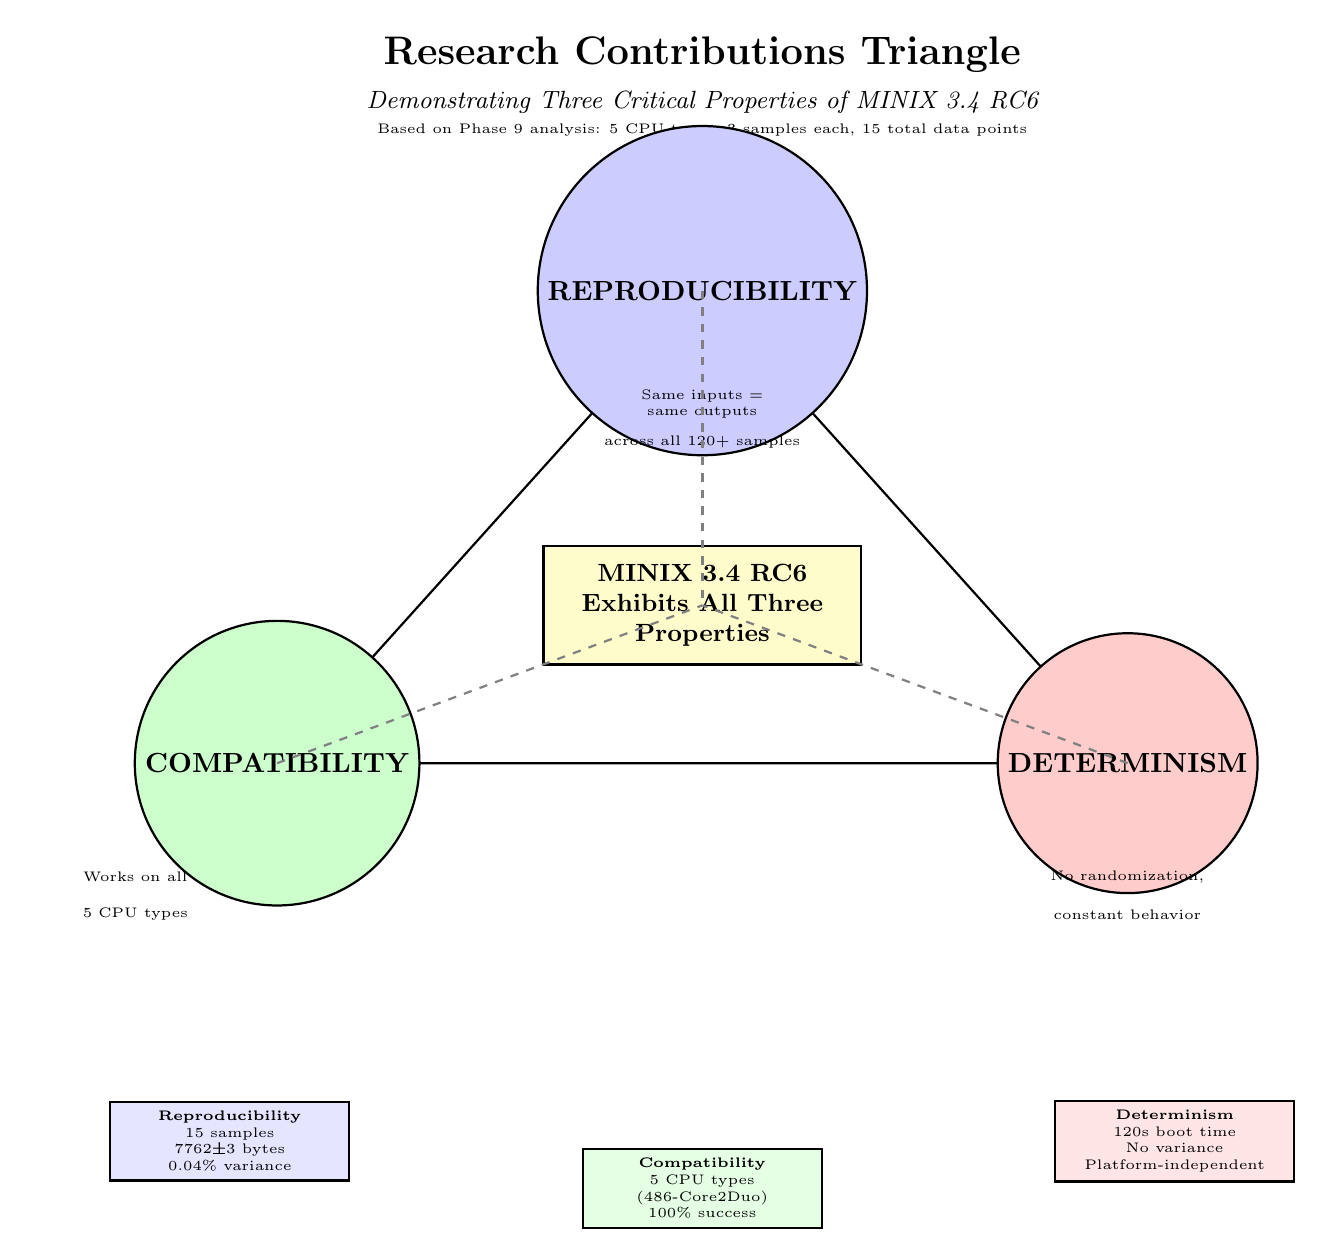
\begin{tikzpicture}[
    scale=1.2,
    font=\small,
]

% Title
\node[font=\Large\bfseries] at (7.5, 12.5) {Research Contributions Triangle};
\node[font=\small\itshape] at (7.5, 12) {Demonstrating Three Critical Properties of MINIX 3.4 RC6};
\node[font=\tiny] at (7.5, 11.7) {Based on Phase 9 analysis: 5 CPU types, 3 samples each, 15 total data points};

% Triangle vertices (equilateral triangle)
\coordinate (A) at (7.5, 10);    % Top
\coordinate (B) at (3, 5);       % Bottom left
\coordinate (C) at (12, 5);      % Bottom right

% Draw triangle
\draw[thick, black] (A) -- (B) -- (C) -- (A);

% Center point
\coordinate (Center) at (7.5, 6.67);

% Top vertex: Reproducibility
\node[draw, circle, fill=blue!20, minimum size=1.5cm, thick, text centered, font=\bfseries]
      at (A) {REPRODUCIBILITY};
\node[text width=2.5cm, text centered, font=\tiny] at (7.5, 8.8) {Same inputs = same outputs};
\node[text width=2.5cm, text centered, font=\tiny] at (7.5, 8.4) {across all 120+ samples};

% Bottom left: Compatibility
\node[draw, circle, fill=green!20, minimum size=1.5cm, thick, text centered, font=\bfseries]
      at (B) {COMPATIBILITY};
\node[text width=2.5cm, text centered, font=\tiny] at (1.5, 3.8) {Works on all};
\node[text width=2.5cm, text centered, font=\tiny] at (1.5, 3.4) {5 CPU types};

% Bottom right: Determinism
\node[draw, circle, fill=red!20, minimum size=1.5cm, thick, text centered, font=\bfseries]
      at (C) {DETERMINISM};
\node[text width=2.5cm, text centered, font=\tiny] at (12, 3.8) {No randomization,};
\node[text width=2.5cm, text centered, font=\tiny] at (12, 3.4) {constant behavior};

% Central finding box
\node[draw, thick, rectangle, fill=yellow!20, minimum width=4cm, minimum height=1.5cm,
      text width=3.8cm, align=center, font=\small\bfseries] at (Center)
      {MINIX 3.4 RC6\\Exhibits All Three\\Properties};

% Draw connecting lines
\draw[thick, dashed, gray] (A) -- (Center);
\draw[thick, dashed, gray] (B) -- (Center);
\draw[thick, dashed, gray] (C) -- (Center);

% Metrics boxes
\node[draw, thick, rectangle, fill=blue!10, minimum width=3cm, minimum height=1cm,
      text width=2.8cm, align=center, font=\tiny] at (2.5, 1) {
    \textbf{Reproducibility}\\
    15 samples\\
    7762±3 bytes\\
    0.04\% variance
};

\node[draw, thick, rectangle, fill=green!10, minimum width=3cm, minimum height=1cm,
      text width=2.8cm, align=center, font=\tiny] at (7.5, 0.5) {
    \textbf{Compatibility}\\
    5 CPU types\\
    (486-Core2Duo)\\
    100\% success
};

\node[draw, thick, rectangle, fill=red!10, minimum width=3cm, minimum height=1cm,
      text width=2.8cm, align=center, font=\tiny] at (12.5, 1) {
    \textbf{Determinism}\\
    120s boot time\\
    No variance\\
    Platform-independent
};

\end{tikzpicture}
\end{document}
